\newpage
\section{Architecture}
Avant m\^eme de commencer le développement du \textit{Bomberman}, il a fallu s'intéresser
sur comment les objets issus de nos différentes classes allaient interagir entre eux. 
Même si cette étape n'est pas fondamentalement indispensable, veiller à adopter un 
\textit{design pattern} structuré s'avère l'\^etre si l'on désire s'affranchir au maximum 
de toute redondance, lourdeur dans la gestion des classes ...

\subsection{Model-View-Controller}
\begin{wrapfigure}[7]{r}{3cm}
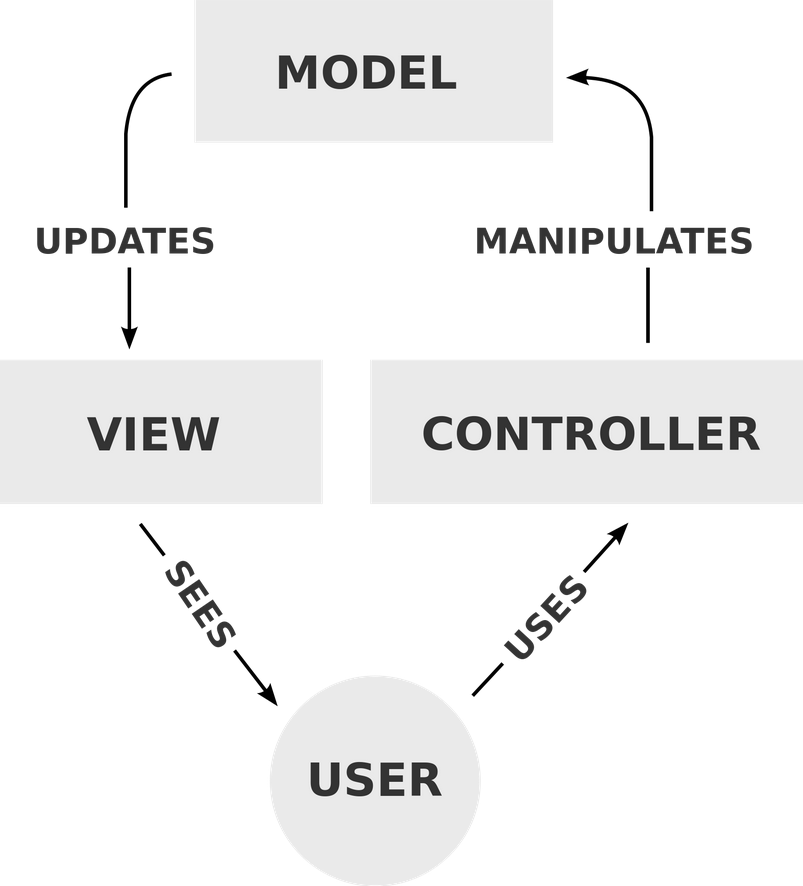
\includegraphics[scale=0.1]{ch1/image1.png}

\captionof{figure}{MVC}
\end{wrapfigure}
Le design pattern que nous avons choisi pour notre projet est le modèle-vue-contrôleur, 
MVC en abrégé. L'intérêt de l'utilisation de ce patron est de séparer notre programme 
en trois parties différentes, ayant chacune un objectif particulier :
\begin{enumerate}
\item Un modèle
\item Une vue
\item Un contr\^oleur
\end{enumerate}\ \\
Le \textit{modèle} se charge de la gestion des données : les objets qui le constituent sont 
chargés de leurs traitements. Après avoir mis à jour les données, le modèle informera la  
vue de se mettre à jour. La \textit{vue} concerne l'interface graphique de notre programme, 
chargé d'interagir avec l'utilisateur. Le \textit{contr\^oleur} reçoit les actions de 
l'utilisateur entrées via la vue. Son but est de vérifier la validité de ces données pour 
ensuite prévenir le modèle d'en prendre compte.\\

La motivation à utiliser ce design pattern découle de la séparation claire entre 
l'interface graphique gérée par la vue et le traitement des données par le modèle. 
Cette séparation rend le développement de l'interface graphique plus simple que si
celle-ci devait être "éparpillée" dans les différentes parties du code. La 
séparation des tâches est un avantage de poids pour ce projet réalisé en équipe : la
répartition des travaux ainsi que la maintenance peut se faire de façon naturelle. De 
plus, "découper" un code en plusieurs parties diminue grandement la complexité générale 
au niveau de la conception.


	\subsection{Implémentation du MVC à notre projet}
		\subsubsection{View}
		Notre \textit{view} se compose de deux classes : 
		\begin{multicols}{2}
        \begin{enumerate}
            \item \texttt{Window}
            \item \texttt{Panel}
        \end{enumerate}
	    \end{multicols}
	    La classe \texttt{Window} hérite de la classe \texttt{JFrame}. C'est elle 
	    qui se charge d'afficher une fenêtre à une taille pré configurée. Le contenu
	    de cette fenêtre est géré par la classe \texttt{Panel} qui hérite de la 
	    classe \texttt{JPanel}. Celle-ci récupère les modifications effectuées par le 
	    modèle après que celui-ci lui ait informé de se mettre à jour pour ensuite 
	    les afficher.
	    
		
		\begin{figure}[H]
        \centering
            \subfigure [View]{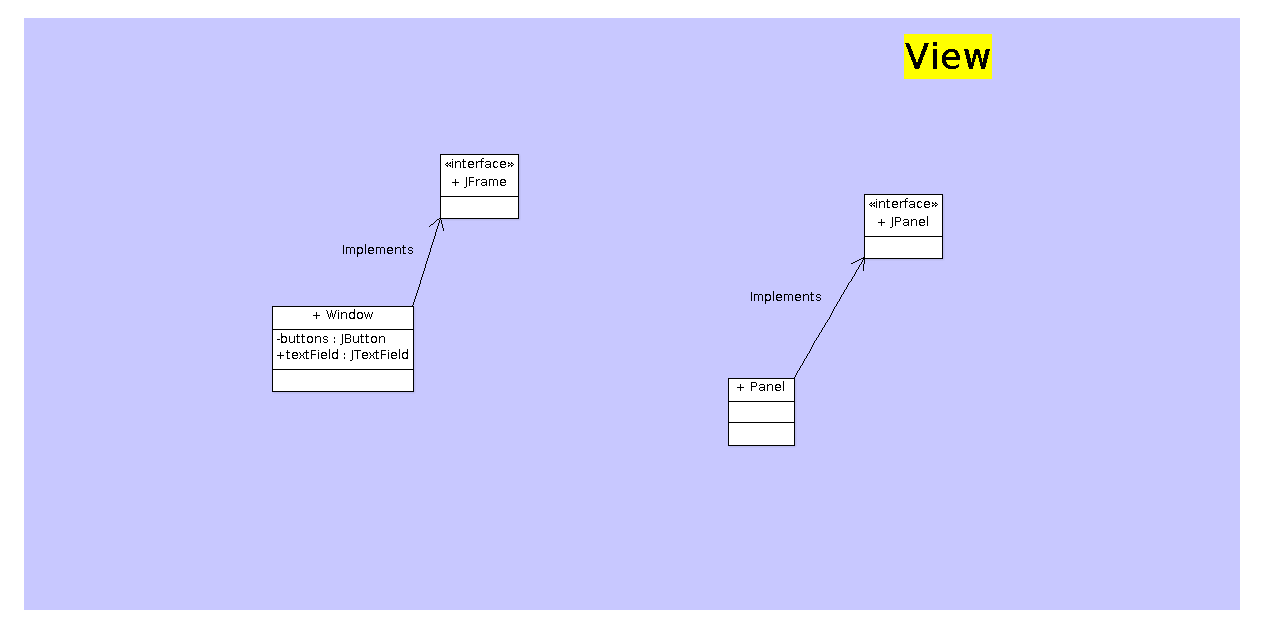
\includegraphics[scale=0.17]{ch1/View}}
        \quad
            \subfigure [Controller]{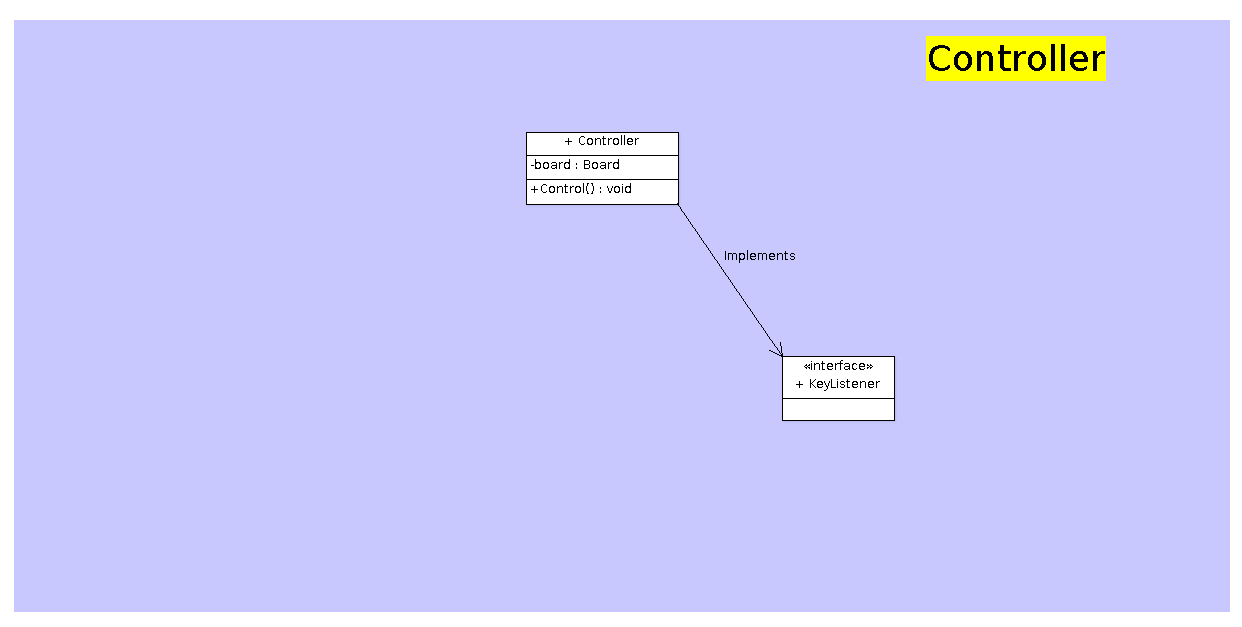
\includegraphics[scale=0.17]{ch1/Controller}}
            \caption {Diagramme des classes : View/Controller}
        \end{figure}		
        
        \subsubsection{Controller}
        Notre \textit{controller} ne se compose que d'une unique classe pour l'instant :
        \begin{enumerate}
        \item \texttt{Controller}
        \end{enumerate}
        S'il n'y a qu'une seule classe, c'est parce que le nombre d'actions 
        susceptibles d'\^etre effectuées par l'utilisateur est assez limité. En effet,
        la classe \texttt{Controller} se contente de récupérer les touches
        rentrées par l'utilisateur (par exemple, les touches directionnelles) et de 
        les transmettre au modèle si cette dernière déclenche bien une action. Cette figure est encore incomplète dans la mesure où il va falloir ajouter les différents \textit{ActionListener}. Ceux-ci concernent les différents boutons qui seront présents dans l'interface graphique avant le lancement du jeu. "L'esthétique" du projet n'ayant pas encore été approfondie, le groupe a préféré garder un modèle purifié, qui sera plus détaillé pour le rapport final.
        
        
        \subsubsection{Model}
        Notre \textit{model} se compose de deux interfaces :
  		\begin{multicols}{2}
        \begin{enumerate}
            \item \texttt{IPlayer}
            \item \texttt{Explosion}
        \end{enumerate}
	    \end{multicols}
	    et de dix classes dont deux classes mère ($\bullet$) où la première est 
	    abstraite. Les implémentations d'interfaces sont représentées par $\rightarrow$, 
	    les classes filles par une sous-liste (-) et l'implémentation d'interface entre
        une classe concrète et une interface par $\twoheadrightarrow$\footnote{Pour 
        plus de clarté, consultez la \autoref{fig:DiagModel}} :
	    \begin{multicols}{2}
        \begin{itemize}

            \item \texttt{Element}
            \begin{itemize}
            \item[$\rightarrow$] \texttt{Explosion}
				\begin{itemize}
				\item[$\twoheadrightarrow$] \texttt{NExplode}
				\item[$\twoheadrightarrow$] \texttt{PExplode}
				\item[$\twoheadrightarrow$]	 \texttt{EBomb}			
				\end{itemize}				            
            
            
	        \item \texttt{Player}
	        \begin{itemize}
	        \item[$\rightarrow$]	 \texttt{IPlayer}	
	        \end{itemize}
            \item \texttt{Bomb}
            \item \texttt{Block}
            \item \texttt{Bedrock}
            \item \texttt{Bonus}
            \end{itemize}
            \item \texttt{Board}
        
        \end{itemize}
        \end{multicols}
        
        La classe avec laquelle notre contrôleur communique est la classe 
        \texttt{Board}. La classe board crée une matrice remplie d'éléments 
        de type \texttt{Element} : joueurs, différents blocs, bombes, etc. 
        Lorsque l'utilisateur demande d'effectuer un déplacement, celui-ci 
        est renseigné à cette classe via le contr\^oleur pour finalement 
        modifier les attributs de positions du joueur. La matrice remise à 
        jour, un message sera envoyé à la vue afin de remettre à jour l'
        interface graphique.\\
        
        Les différents composants de notre classe \texttt{Board} sont tous 
        de types \texttt{Element}. La classe \texttt{Element} possède cinq 
        classes filles : \texttt{Player, Bomb, Block, Bedrock, Bonus}. Le 
        nom des classes est assez explicite si ce n'est pour les deux classes 
        chargées de la gestion des blocs :
        \begin{enumerate}
        \item \texttt{Block} : une case pouvant \^etre détruite suite à l'
        explosion d'une bombe.
        \item \texttt{Bedrock} : une case ne pouvant \^etre détruite (ainsi 
        qu'une petite référence à \textit{Minecraft}).
        \end{enumerate}
        
        Afin de gérer les explosions de façon la plus efficace que possible, 
        la méthode \texttt{explode()} a été définie au sein de la classe 
        \texttt{Element}. Or, cette méthode n'a pas le même comportement pour
        un objet de la classe \texttt{Bedrock} que pour un de la classe \texttt{Bomb} mais a le m\^eme pour un objet de la classe \texttt{Bonus}. 
        Afin que cette méthode puisse être utilisée de façon polymorphe et pour
        éviter les doublons de code, l'interface \texttt{Explosion} implémentée 
        à \texttt{Element} permet de définir un comportement adapté à l'objet
        concerné.\\
        
		Cependant, la classe \texttt{Player} doit posséder des attributs et 
		des méthodes que les autres classes héritant de \texttt{Element} ne 
		possèdent pas. Afin de conserver le polymorphisme, l'interface 
		\texttt{IPlayer} a été implémentée à notre classe \texttt{Player}.
        
        \begin{center}
		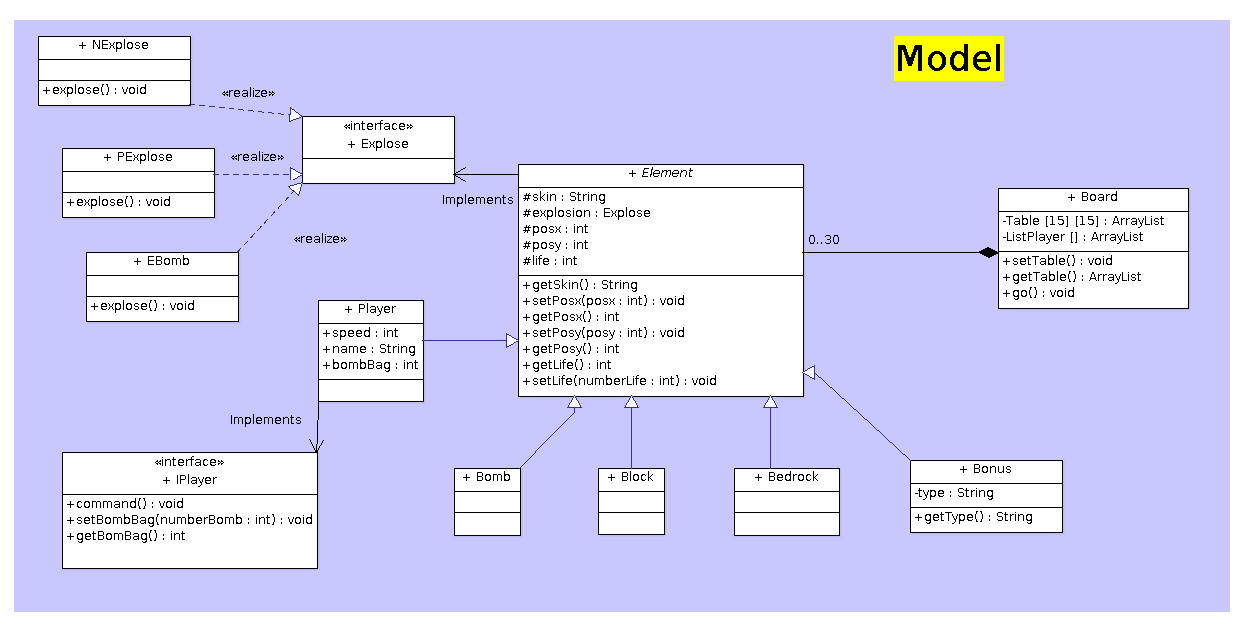
\includegraphics[scale=0.35]{ch1/Model}
 	 	\captionof{figure}{Diagramme les classes : Model}
 	 	\label{fig:DiagModel}
        \end{center}
        
        
        
        
        
        
        
        
        
        
        
        
        
        
        
        
        
        
        
        
        
        
        
        
        
        
        
        
        
        
		
	